\documentclass{article}
\usepackage{graphicx} % Required for inserting images
\usepackage{enumitem} % for customisible enumerators
\usepackage{float} % for text under pictures
\usepackage[colorlinks=true, linkcolor=black]{hyperref} % for links in refs
\usepackage{cleveref} % for easier referencing
\usepackage{caption} % easier captioning for tables
\captionsetup[table]{position=above}

\title{Vilnius University\\Faculty of Mathematics and Informatics\\Software Engineering\\3rd course\\[1cm] \Huge Universal PoS application for small to medium-sized businesses\\[1cm]}
\author{\textbf{PoS application [Tuesday 12 pm]}\\[0.25cm]Rytis Tauras\\Matas Čeplinkas\\Emil Duko\\Žygimantas Vidmantas\\Rytis Jonika\\[4cm]}
\date{September 2025}

\usepackage{titlesec}
\newcounter{subsubsubsection}[subsubsection]
\renewcommand\thesubsubsubsection{\thesubsubsection.\arabic{subsubsubsection}}

\newcommand\subsubsubsection[1]{
  \refstepcounter{subsubsubsection}
  \paragraph{\thesubsubsubsection\quad #1}
}

\begin{document}

\maketitle

\newpage
\setcounter{tocdepth}{3}
\tableofcontents
\newpage

\section{Introduction}
\subsection{Software title}
\subsubsection{Full title} Universal PoS application for small to medium-sized businesses
\subsubsection{Short title} PoS application
\subsection{Problem statement}  Today, the need for a reliable point-of-sale (PoS) system is greater than ever before. Due to fast pace and increasing client traffic, companies and their employees who use PoS systems face the challenge of unreliable and inefficient systems.
\par To be more precise, PoS operators that work hand in hand with the system often struggle with unexpected errors, lack of functionality, difficult to navigate user interfaces, slow processing, and inefficient workflow, all of which cause unwanted stress on a daily basis. Furthermore, it also has a negative effect on new business owners because starting a business takes more time, and usually they have to sort through different systems to find the best fit, which results in significant part of resources being used for installation and employee training. The clients of these companies expect an excellent quality of service, and these faulty systems directly contribute to longer wait times and a general decrease in the quality of the provided service.
\par Challenges mostly arise in cafes, bars, restaurants, spas, and other settings, where smooth workflow between sales, reservations, and management is crucial - the hospitality sector. Firstly, the root of the problem usually lies in poor synchronization between different departments, for example, the system fails to notify that a product is out of stock and the product is ordered anyway. Secondly, most PoS systems support only a single language menu or user interface, which causes problems for international workers, with another problem being confusing or unintuitive user interfaces.
\par All of these problems occur during work or preparation hours, which causes delays and mistakes. It is important to address this issue because faulty PoS systems hinder business processes resulting in financial losses. It also reduces customer satisfaction, causing customers to develop mistrust, which creates barriers for new businesses or increases frustration for more established business owners and their employees.
\newpage

\section{User needs analysis}
\subsection{Expectations of the stakeholders}
\subsubsection{Primary stakeholders}
\textbf{PoS operators} expect to have a system for creating orders and making appointments that:
\begin{itemize}
    \item Has high transaction efficiency
    \item Reduces errors
    \item Helps provide quick assistance to customers
    \item Requires minimal training and is easy to remember
    \item Has smooth integration of appointment system
    \item Allows resource monitoring
    \item Supports card, cash, and gift-card payments
    \item Supports multiple languages.
\end{itemize}


\subsubsection{Secondary stakeholders}

\textbf{Clients} expect the orders or appointments to be accurately delivered and without delays, as well as to have an option of splitting the bill, receiving an invoice, or refunding an order or service. Clients expect to be reminded of their upcoming appointments.
\textbf{\\ \\Other employees} expect to have a system that allows them to view appointments assigned to them on their own devices and be notified on any changes.
\textbf{\\ \\Business managers} require an intuitive system to manage product or menu items, inventory, and discounts.

\subsubsection{Tertiary stakeholders}

\textbf{Business owners} expect a system that serves customers faster, is error-free, is adaptable to their business model, can be integrated into current systems and into current workflows seamlessly, and does not require lengthy training sessions for PoS operators.
\newpage

\subsubsection{Competitors}The closest competitors rivaling with our PoS application are:
\begin{itemize}
    \item \textbf{Paysera PoS}
    \\Paysera PoS is a widely applicable, feature-rich system with an intuitive and modern user interface.
    \item \textbf{WinPoS}
    \\WinPoS offers installation with Windows Embedded PoSready system, and offers multi-language support.
    \item \textbf{iiko}
    \\iiko offers multiple restaurant-oriented PoS systems according to the specific process, and offers comprehensive operation statistics to the customer.
    \item \textbf{r\_keeper}
    \\r\_keeper offers a simplistic PoS system for restaurants with an updated user interface.
    \item \textbf{nSoft nPoint}
    \\n\_soft provides a comprehensive PoS system for many organization types, with support for third-party programs.
\end{itemize}
The main advantages of our PoS application are: multi-language UI support (beyond Lithuanian and English), the ability to translate menus, an easier to learn user interface and a more affordable service.
\subsubsection{Developers \& maintenance team}
Team responsible for maintenance and development expects a system that can be scaled or adjusted if business model of PoS system's customer changes. Additionally, it should be maintainable without dedicating more than one person to keep things running.  
\newpage
\subsection{PoS operators research}
\subsubsection{Current users' activities}

\subsubsubsection{Unknown language borders}
\label{Unknow language borders}
\paragraph{\small Story:} Carlos and Juan, two older gentlemen from Spain, have joined a popular Lithuanian specialty coffee place. Both of them speak Spanish, Carlos knows English. They have extensive knowledge about coffees and more than 30 years of experience in the field. This experience does not translate well to their order taking speed, as the system only has English and Lithuanian user-interface options, and the menu of beverages and food items is available only in Lithuanian language. Carlos has set the user interface to English, so he has no problem understanding the system's order flow, but both Carlos and Juan struggle with selecting items from the Lithuanian menu in the system. Despite their experience, this has significantly impacted their work efficiency. Instead of a few seconds to add an item to an order on the touch screen PoS system, while they learn the menu, it takes more than 20 seconds to remember the item's name in Lithuanian language. Juan struggles with remembering different terms in the check out menu. He has learned basic order flow (creating a new order, selecting payment, etc), but when he needs to perform a rare action (such as refunding or splitting the order), he gets stuck and needs to get help from other employees. The average total order taking time increases from less than a minute to over 2 minutes (Not counting time to make and serve the order). The coffee place sells hundreds of beverages and other items per day, and this delay adds up to a significant amount causing slower service and dissatisfied customers.

\paragraph{\small Problems and Opportunities:} The problem is caused by the fact that the current PoS system only supports a single language item menu and a two-language user interface.\\ An opportunity would be to develop a system with a broad selection of languages for the user interface and an option to add translation to the menu items in the needed language.

\subsubsubsection{Stock management failure}
\label{Stock management failure}
\paragraph{\small Story:} Twenty-year-old student Laura is a new hire in a take-away burger joint. After a short introduction to the PoS system, she starts taking customer orders. It is a busy Friday night. She listens to an order from a customer and enters it into the system, a burger with cheese and bacon. The customer leaves and waits for the order outside of the restaurant. Laura starts taking another customers' orders, when 10 minutes later an angry cook comes out to the front and shouts at Laura that they are out of bacon and that she should have asked them before confirming the order. Now Laura needs to run outside, find the customer and ask them to order again while the previous order is refunded, or to get a partial discount and get the burger without bacon. The customer is angry, since they have already waited a total of 15 minutes and requests a refund. While Laura tries to de-escalate the situation a long, noisy queue forms.
\paragraph{\small Problems and Opportunities:} The problem was caused by the fact that the current PoS system does not have an integrated stock management system.\\ An opportunity would be to design the system that would track the inventory. Additionally, the system should also support refund management, if the customer is unsatisfied with the service.

\subsubsubsection{Failed customer assistance}
\label{Failed customer assistance}
\paragraph{\small Story:} Trevor is a fifty-year-old who works in a restaurant part time. While getting an order he gets asked about the list of ingredients used in the cake that the customer wants to order, specifically whether it contains any traces of nuts because the customer is severely allergic to them. Trevor is not sure about the answer, so he tries looking for that information in his ordering system, but cannot find it. He struggles with handling the system, because he did not grow up with this kind of technology at hand. Then he decides to go to the product manager for more information, however his office is in the back corner of the restaurant so Trevor has to go through the kitchen to reach it. This action results in Trevor having to drop his work and taking up 5 minutes of his and the customer's time while also hindering the build of trust between restaurants' customers.
\paragraph{\small Problems and Opportunities:} The problem was caused by not having means to get additional information (ingredients and descriptions) in the PoS system or having it implemented in a way that inexperienced PoS operators could not find it.\\ An opportunity would be to design the PoS system that has easy to find information to any anticipated questions that the customer might come up with without having to involve any other employees.

\subsubsubsection{Receipt management}
\label{Receipt management}
\paragraph{\small Story:} Renata is a 32-year-old waiter working in a restaurant. During a business meeting, one of the two attending parties, in a hurry, requests to pay and have the bill split according to the ordered food, and have an invoice sent to their e-mail. The in-use PoS system, "nPoint", supports only receipt splitting, but not forwarding invoices through e-mail. Because of this, Renata has to inform the customers that the invoice can only be printed out, or that they can manually send an e-mail in one to two business days. The customer has to choose the inconvenience of waiting for the invoice to arrive, or take the printed invoice, and risk damaging or losing it. The customer chooses to take the physical invoice, and is dissatisfied with the restaurant.

\paragraph{Problems and Opportunities:} The problem arises when clients request an invoice for their order in a non-physical format, a feature only supported by one other provider, which does not fit the needs of the restaurant.\\The ability to send invoices through e-mail in the PoS application is a great option when the customer is short on time, and generally is more convenient than a printed invoice. An additional opportunity is to have support for order-splitting at any given time during the orders lifespan, as customers may request to pay and leave separately.

\subsubsection{Characteristics of people, activities, context, and technologies}
\paragraph{\small People:} Mostly young hospitality workers varied in ethnic backgrounds who have high motivation to succeed, with the exception of elderly personnel, who are not so handy with technology, some of whom lack sufficient training or struggle with the language barrier of the system.
\paragraph{\small Activities:} Daily high pressure and quick response time work consisting of handling order input and searching for important information - sometimes stressful safety-critical situations where customers' health could be at risk. The main goal is to do your job as quickly and as correctly as possible.
\paragraph{\small Context:} Physical environment is loud, warm or even hot near the kitchen area, filled with a variety smells and noises. The space where the workers manage orders system is well lit, but the main dining area is lit quite dimly. Social environment consists of constant interactions with customers and colleagues as well as individual concern of getting orders correctly.
\paragraph{\small Technologies:} A touch screen interface facing the worker to input orders, edit them or close tabs. Printer for checks and hand card terminal for cashless transactions.

% add main functions like login and cancel, refund etc (function list)
\subsubsection{Needs}
\label{N1-10}
\begin{enumerate}[label=N\arabic*.]
    \item Carlos and Juan need item menu translation functionality in the PoS system, so they would not need to learn and remember foreign language names during  working hours. This would significantly increase their productivity.
    \item Juan needs a wide user-interface language selection (at least 5 widely used languages), to ensure his work does not get obstructed of a language barrier during order taking, especially with unusual requests.
    \item Carlos and Juan need to be able to use the search to find items in their native language, so they can find items quickly and without the need to memorize foreign item names.
    \item Laura needs to be able to see the remaining product stock during order entry into the system. She would not have to confirm with cooks that there are enough products for the order, saving both her and the customers time.
    \item Laura needs a feature to enter the remaining product stock during stock-taking or when needed so that an accurate inventory situation is portrayed during service hours, in order to know which items are still available for sale.
    \item Laura needs a feature that decrements the remaining product stock after each sale made during service and gives a warning when certain items reaches a set (adjustable) near out-of-stock amount. This would prevent selling an item that is out of stock or near it without noticing.
    \item Laura requires refund support, as the customer may request a refund if they are not satisfied.
    \item Trevor needs the ability to access information about menu items, such as their ingredients and descriptions, so he could provide feedback to customers' questions without having to ask the manager.
%    \item Trevor needs an understandable interface to retrieve information about menu items, so he can quickly find and provide needed information to the inquiring customer. 
    \item Renata needs to be able to quickly generate an invoice for a specific order and have options to print out or send the receipt according to customer request.
    \item Renata needs a capability to swiftly split up a specific order into multiple orders at any given time in during order taking.
\end{enumerate}

\begin{table}[h]
\centering
\caption{Traceability matrix for PoS operators needs and stories they stem from}
\begin{tabular}{|c|c|}
\hline
\textbf{Need ID} & \textbf{Story number} \\ \hline
N1  & \ref{Unknow language borders} \\ \hline
N2  & \ref{Unknow language borders} \\ \hline
N3  & \ref{Unknow language borders} \\ \hline
N4  & \ref{Stock management failure} \\ \hline
N5  & \ref{Stock management failure} \\ \hline
N6  & \ref{Stock management failure} \\ \hline
N7  & \ref{Stock management failure} \\ \hline
N8  & \ref{Failed customer assistance} \\ \hline
N9  & \ref{Receipt management} \\ \hline
N10 & \ref{Receipt management} \\ \hline

\end{tabular}
\end{table}

\subsubsection{Usability objectives}
\begin{enumerate}[label=UO\arabic*.]
    \item Learnability: 95\% of foreign workers will be able to perform the basic and unusual PoS flows (order taking, different payment methods, refunds, check splitting, etc.) in their first usage session in less than 1 hour of training/usage, if the user interface and item menu supports their native language.
    \item Satisfaction: At least 80\% of foreign PoS system operators will rate the system as 'satisfactory' or better (more than 4 on a 5-point scale) after a week of work with the system, if it is available in their language.
    \item Memorability: At least 95\% of foreign workers will be able to complete unusual tasks during service (refunds, check splitting, providing information) after not using the PoS system for more than a week.
%    \item Errors: If the inventory amounts are entered correctly, 100\% of the orders taken by the PoS operator will reach the buyer (having enough stock).
    \item Efficiency: PoS system operating employee should be able to find an answer to a question in 30 seconds or less, if the information is disclosed in the system.
    \item Learnability: 90\% of Employees should be able to learn the use of system's basics in 30 minutes or less.
    \item Learnability: At least  90\% of PoS operators that have received 30 minutes of training on the system will be able to split an order by customers request and send an invoice to their e-mail address, if needed.
\end{enumerate}

\begin{table}[h]
\centering
\caption{Traceability matrix for usability objectives and stories they stem from}
\begin{tabular}{|c|c|}
\hline
\textbf{Usability objective ID} & \textbf{Story number} \\ \hline
UO1  & \ref{Unknow language borders} \\ \hline
UO2  & \ref{Unknow language borders} \\ \hline
UO3  & \ref{Unknow language borders} \\ \hline
UO4  & \ref{Failed customer assistance} \\ \hline
UO5  & \ref{Failed customer assistance} \\ \hline
UO6  & \ref{Receipt management} \\ \hline
\end{tabular}
\end{table}

\newpage
\subsection{Clients research}
\subsubsection{Current users' activities}
\subsubsubsection{Customer frustration}
\paragraph{\small Story:} Mark is an electrician in his thirties, who has a short lunch break of 30 minutes, during his workday. For that reason, he needs his meal served within 15 minutes, so that he has a reasonable amount of time to eat. After coming to a restaurant near his workplace, an employee takes his order. The employee responsible for operating the PoS system is new and takes about 5 minutes to put in the order. For that reason, Mark has to rush his meal and is unsatisfied with the restaurant.
\paragraph{\small Problems and Opportunities:} The problem is that the customer, who is in a hurry, did not get the best possible delivery speed, which caused him frustration.\\ An opportunity would be to design an interface that is as simple as possible for as many people as possible, which would be achieved by testing the system with people who are unfamiliar with it.

\subsubsection{Characteristics of people, activities, context, and technologies}
\paragraph{\small People:} A customer who is a physically average, healthy adult. He is in a rush due to the limited time in lunch break.
\paragraph{\small Activities:} Ordering food is a very simple, well defined task that has clear steps and occurs frequently. High time pressure because it needs to be in time with the customer's lunch break.
\paragraph{\small Context:} The restaurant's environment is moderately noisy, many people due to lunch time. Individual activity is dependent on staff(organization).
\paragraph{\small Technologies:} No technologies used, but customer is affected by systems that influence the efficiency of food delivery process.

\subsubsection{Needs:} Needs will not be discussed, because the customer does not interact directly with the system.
\subsubsection{Usability objectives:} Usability objectives will not be discussed, because the customer does not interact directly with the system.

\newpage
\subsection{Other employee research}
\subsubsection{Current users' activities}
\subsubsubsection{Employee stress}
\paragraph{\small Story: } Sarah is a hairdresser in her twenties, who works for a company offering hairdressing services and gets many appointments every day. Every time she wants to know her schedule, she has to go to a receptionist who is on a different floor and ask for it regularly. Additionally, it is hard for her to know when her schedule gets updated, which happens frequently - whenever any customer makes an appointment. This causes her additional work-place stress and tires her out. 
\paragraph{\small Problems and Opportunities:} The main problem is that there is no way for an employee to quickly check their schedule that rapidly changes, from their own devices, which leads to them getting stressed.\\ An opportunity would be to implement a system, that would allow an employee to check their schedule easily near their workplace, using a personal computer or other device.

\subsubsection{Characteristics of people, activities, context, and technologies}
\paragraph{\small People:}  An employee who is a young adult. Physically average, healthy adult and has a high motivation to learn new technology to improve work efficiency. Intermediate technological ability: not an expert, but can adapt to new technologies.
\paragraph{\small Activities:} Checking daily appointments - simple and very frequent activity. The activity takes a relatively low amount of time - a few minutes to go and talk to a receptionist, but has a high time pressure, considering customers might be waiting.
\paragraph{\small Context:} Standard office environment, busy atmosphere. Individual activity, dependent on receptionist located in a different area.
\paragraph{\small Technologies:} No technologies used, manual communication with receptionist.
% should we mention standart hairdressing technologyy like blowdryer, trimmer etc?

\subsubsection{Needs:}
\label{N11-12}
\begin{enumerate}[label=N\arabic*.]
\setcounter{enumi}{10}
\item Sarah needs to be able to easily check up-to-date scheduled appointments before and during work hours in her own device so that she doesn't have to go to a receptionist and waste time and energy.
\item Sarah needs notifications (e-mails or text messages) immediately sent to her device whenever her schedule changes.
\end{enumerate}

\subsubsection{Usability objectives}
\label{S7-9}
\begin{enumerate}[label=UO\arabic*.]
\setcounter{enumi}{6}
    \item Efficiency: Hairdressers will be able to check their up-to-date schedule in under 30 seconds, compared to several minutes walking to a receptionist.
    \item Memorability: 90\% of hairdressers (or other service providers) who have not used the system for 2 weeks will be able to check and understand their schedule in less than 1 minute without retraining.
    \item Learnability: 95\% of hairdressers (or other service providers) will be able to view, navigate and understand their appointment schedule within 5 minutes of first using the system.
\end{enumerate}

\subsection{Business manager research}
\subsubsection{Current users' activities}
\subsubsubsection{Manual labour}
\paragraph{\small Story: } Janina, a middle-aged manager at a restaurant, received a shipment of new products today. To promote these new items, she was instructed to apply discounts. Each time, she has to calculate the reduced prices herself, update them in the system one by one, and later restore the original prices after the promotion ends. Once the campaign is over, Janina needs to know how many of the new items were sold in order to report how well the products were received. To do this, she will have to perform a manual inventorisation during closing hours, leaving her overworked and unhappy.

\paragraph{\small Problems and Opportunities:} The core issue is the manual nature of the discounting process. Janina has to calculate reduced prices herself, enter them into the system one by one, and later restore the original prices once the promotion ends, which is repetitive, time-consuming, and prone to mistakes. In addition, she has no automated way of tracking how many promotional items were sold, forcing her to perform manual inventorisation during closing hours. This adds to her workload and stress. An opportunity would be to implement a system that allows time-limited discounts that automatically revert to the original price once the promotion period ends, with the ability to apply them in bulk across multiple items. Furthermore, adding built-in inventory tracking would eliminate the need for manual inventorisation, provide immediate insights into campaign performance. Such a solution would reduce human error, save significant time, and increase staff morale by minimizing unnecessary manual tasks.

\subsubsection{Characteristics of people, activities, context, and technologies}
\paragraph{\small People:} A middle-aged manager, with significant knowledge of the system.
\paragraph{\small Activities:} Individual, well defined, frequent, highly repetitive tasks, which could take anywhere from 30 to 180 minutes combined depending on the number of items. Each required item must be assigned a new price twice which is calculated by the manager. Once the changes are saved, the PoS operator can see the new prices. Afterwards she needs to calculate how many items were sold and report that to upper management.
\paragraph{\small Context:} Discounting is an individual activity, however the manager might be disrupted during this work which would highly increase the mistake count when automation is lacking. Inventorisation could be an individual activity, but might also be a group task. However, the fact that it is done during closing hours means that the sun has set and it is darker than usual, meaning that counting errors can happen easily.
\paragraph{\small Technologies:} A standard PoS device - a stationary computer or a tablet.


\subsubsection{Needs}
\label{N13-16}
\begin{enumerate}[label=N\arabic*.]
\setcounter{enumi}{12}
    \item Janina needs to be able to set time-limited discounts on the PoS system during promotional periods, so she would not have to adjust the price back to the original state after the discount is over.
    \item Janina needs to be able to discount multiple items simultaneously, so she would not have to waste time doing it manually on each item separately.
    \item Janina needs discounts to be automatically calculated on discounted items, for example -10\% on coffees for a week, so that she does not have to calculate it by hand and potentially make errors and waste her time.
    \item Janina needs an accurate and reliable inventory management functionality.
\end{enumerate}

\subsubsection{Usability objectives}
\begin{enumerate}[label=UO\arabic*.]
\setcounter{enumi}{9}
    \item Efficiency: Managers will be able to apply discounts to multiple items at the same time in under 2 minutes, compared to 15 minutes for the same count of items, when manually adjusting each item.
    \item Efficiency: Manager setting a promotional campaign (for example, -10\% on all coffees for 1 week) will take less than 2 minutes 90\% of the time.
    \item Memorability: Managers who have not used the system for longer than 1 month will be able to apply discounts in less than 3 minutes without retraining.
    \item Errors: Fewer than 10\% of cases of applying discounts will be set incorrectly (due to user error). 90\% of managers will be able to correct the errors (wrong time frame, items or discount amount) in less than 3 minutes.
    \item Efficiency: Manual stock management will be reduced to the absolute minimum, limited only to essential validation steps such as confirming stock levels before reordering.
\end{enumerate}

\subsection{Additional needs}
After our research, the client has requested additional requirements that were not observed in earlier field research sections. This section includes needs and usability objectives that arise indirectly from customers and those that are used for additional system management.


\subsubsection{Needs}
\label{N17-25}
\begin{enumerate}[label=N\arabic*.]
\setcounter{enumi}{16}
    \item Appointment notifications: right after registering and a day before the appointment, the system must send an SMS message confirming it and reminding the customer.
    \item Appointment modifications: employees must be able to cancel or modify appointments on customer request, ensuring customer satisfaction.
    \item Tax management: authorized employees can create, edit and delete tax records (e. g., VAT).
    \item Schedule management: authorized employees can edit employee work schedules.
    \item Gratuity management: authorized employees can create, edit and delete service charges.
    \item Menu management: authorized employees can create, edit and delete menu items, their variations and bundles. 
    \item Employee management: Only the owner can add, remove or edit employees of their business. 
    \item SuperAdmin: account with SuperAdmin privileges can edit anyone (e. g., add a new business with relevant details, such as contact information, owner user, name).
    \item Payment method support: The system must support multiple payment methods, including cash, card, and gift cards.
\end{enumerate}

\subsubsection{Usability objectives}
\begin{enumerate}[label=UO\arabic*.]
\setcounter{enumi}{14}
    \item Efficiency: PoS system operator after getting familiar with the system should be able to fill in the order in less than 2 minutes on average.
    \item Learnability: 90\% of users should be able to configure taxes, discounts, or product variations within their first use of the system.
    \item Error Prevention: System must prevent changes to historical records (e. g., modifying taxes or service charges should never alter past records).
    \item Satisfaction: At least 80\% of business managers should rate system management functions as “satisfactory” (more than 4/5) after one month of use.
    \item Error Prevention: The system must prevent accidental cancellation or modification of the appointments without confirmation by the employee.
\end{enumerate}


\subsection{Inspiring user interface designs}
\subsubsection{R\_keeper PoS for restaurants}
\begin{figure}[H]
    \centering
    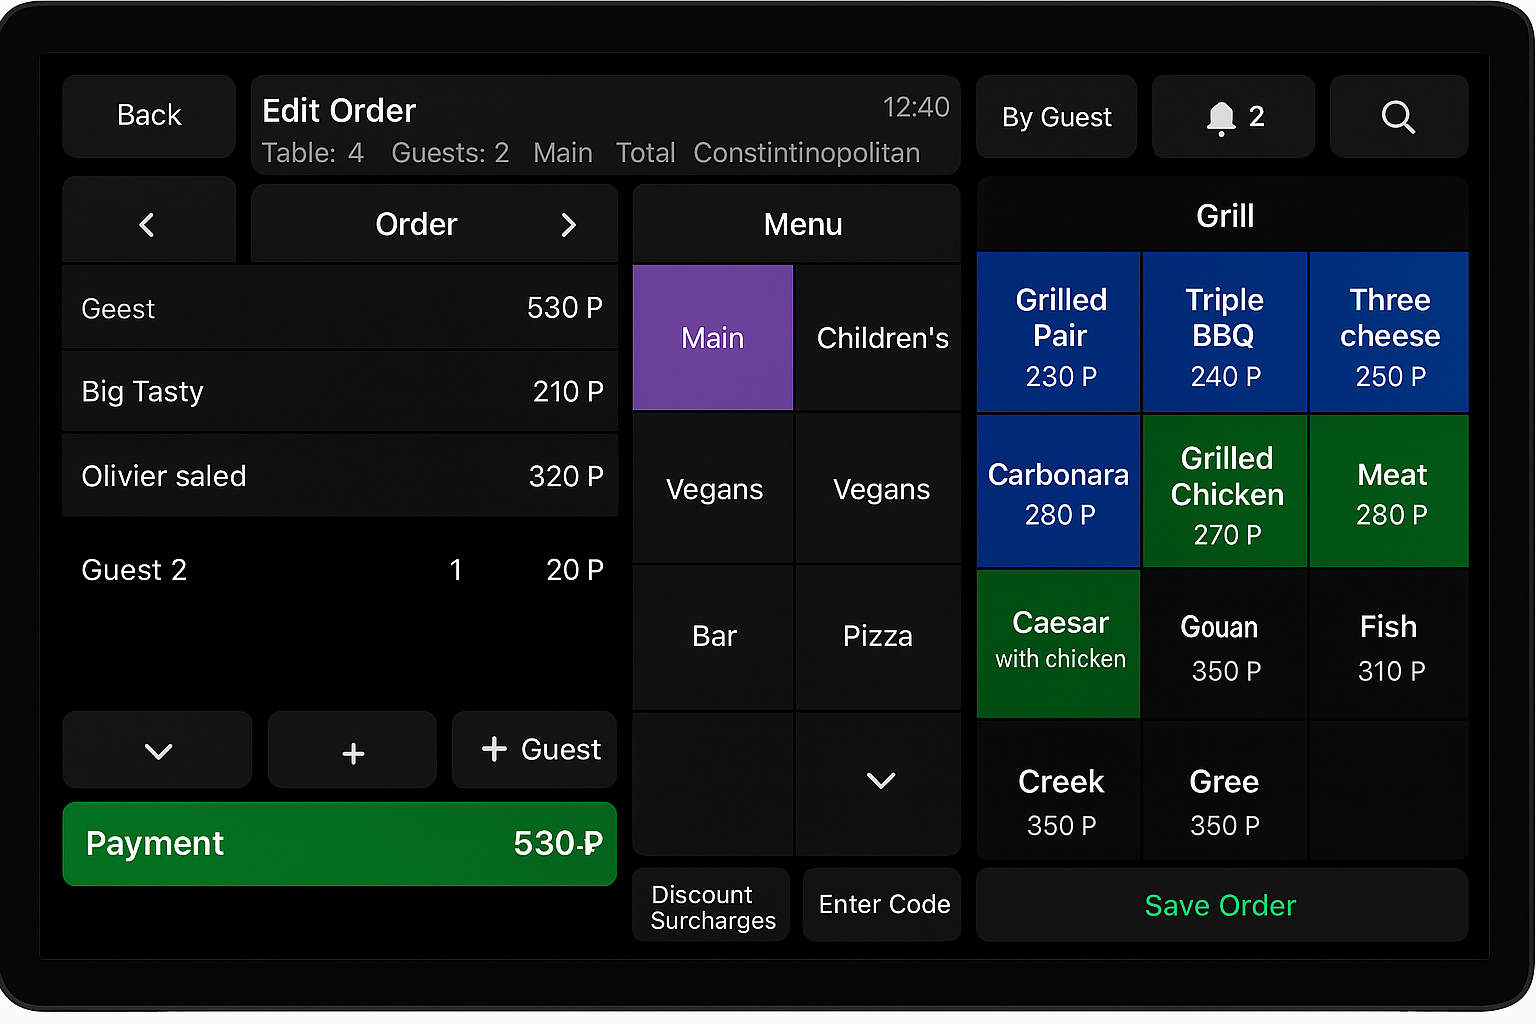
\includegraphics[width=0.9\linewidth]{HCI/images/rkeeper.png}
    \caption{https://www.artlebedev.com/rkeeper/interface/}
    \label{fig:restUI1}
\end{figure}
\noindent
Design in the \cref{fig:restUI1} belongs to one of our competitors - r\_keeper. The design provides all basic functions needed for a restaurant system. However, what is important for us is that information bar at the top suggests that orders are based on individual tables and each table has a number of guests whose orders are separated, but come out to the same bill, while not visible but likely providing the option to split the bill later by each guest. [\cref{N1-10}: N10] Also a search option for the menu at the top right corner. [\cref{N1-10}: N3]

\subsubsection{Restro POS-more detailed and visual restaurant PoS}
\begin{figure}[H]
    \centering
    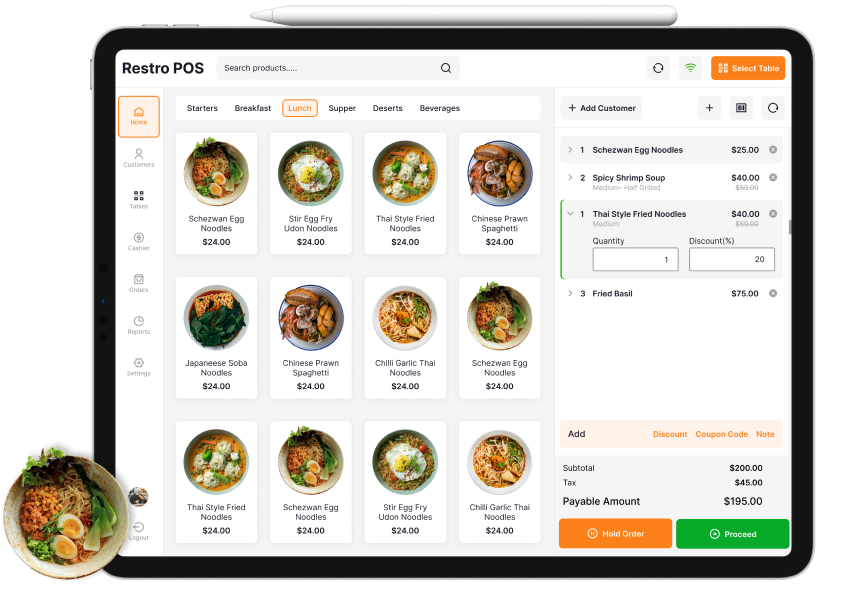
\includegraphics[width=0.9\linewidth]{HCI/images/restaurant_UI_2.png}
    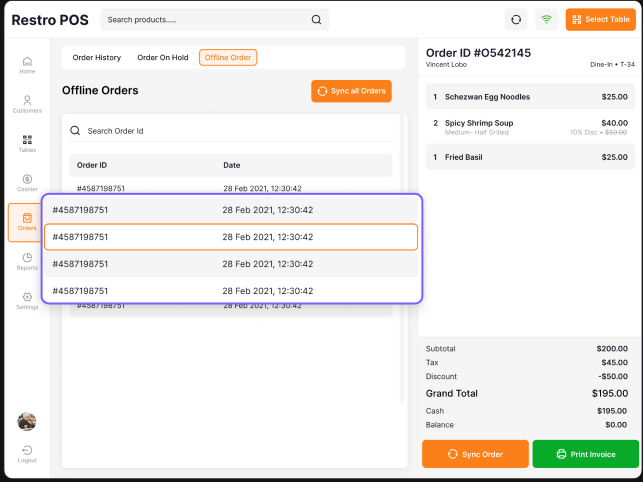
\includegraphics[width=0.8\linewidth]{HCI/images/invoice.png}
    \caption{https://webkul.design/project/pos/}
    \label{fig:restUI2}
\end{figure}
\noindent
In the \cref{fig:restUI2} top image the restaurant system design provides more visual menu items, what could help in memorizing the menu faster for new employees. It also provides the option to enter a discount amount as percentage that the system would calculate and apply to an item. [\cref{N13-16}: N15]\\ In the bottom image of \cref{fig:restUI2} system provides search bar for orders based on their id where one can select an order and print its invoice by pressing the button on the lower right side. [\cref{N1-10}: N9]

\subsubsection{Booker-spa PoS for service booking}
\begin{figure}[H]
    \centering
    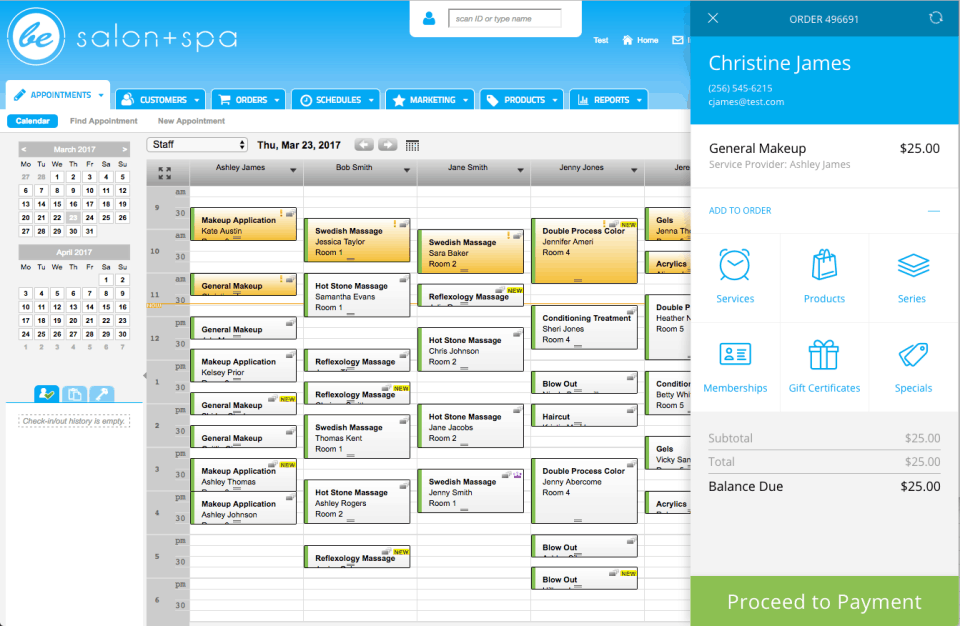
\includegraphics[width=0.9\linewidth]{HCI/images/spa.png}
    \caption{https://www.softwareadvice.com/medical/booker-profile/}
    \label{fig:cafeUI}
\end{figure}
 \noindent
 In the \cref{fig:cafeUI} the spa booking system design provides option to pick any day on the calendar and make a time table appointment for specific employee based on the services they provide. The customer and order details are shown in the menu on the right side, where it is possible to modify it.[\cref{N11-12}: N11, N12; \cref{N17-25}: N18, N20][\cref{S7-9}: UO7, UO8, UO9]

\subsubsection{Inventory management UI for PoS}
\begin{figure}[H]
    \centering
    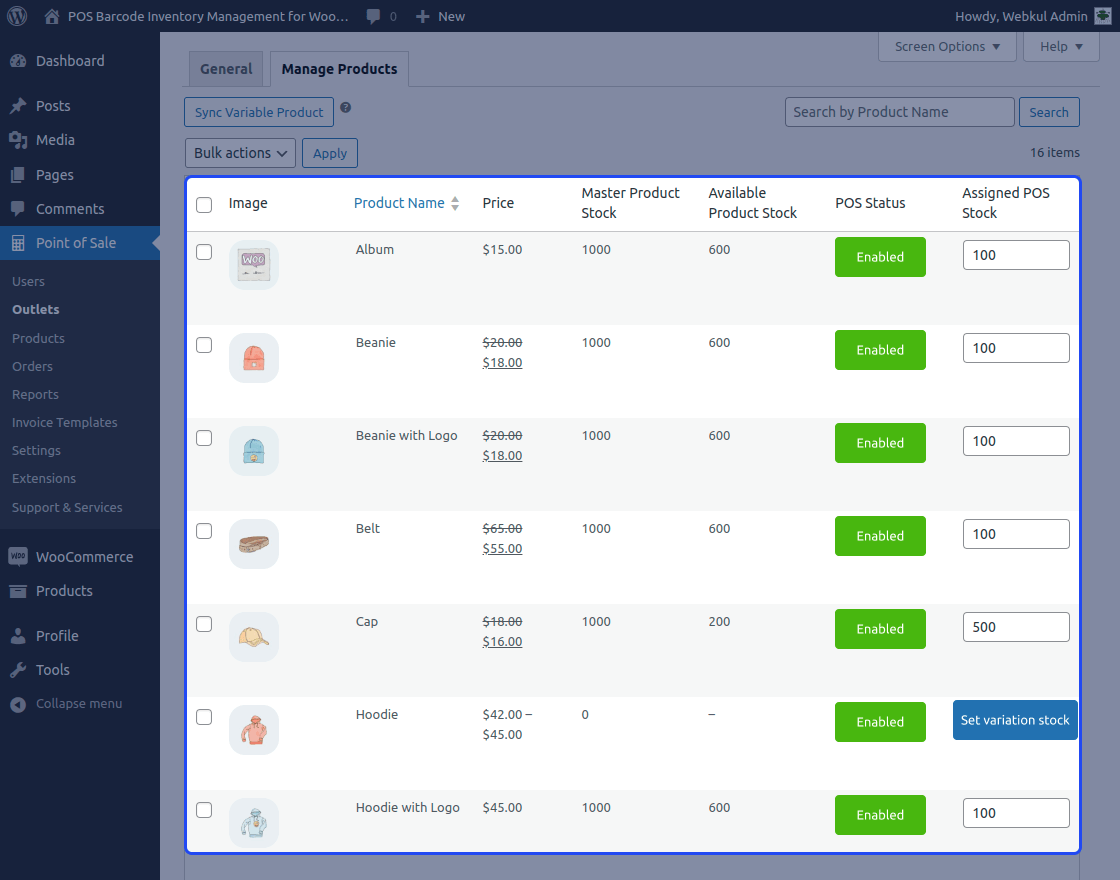
\includegraphics[width=0.9\linewidth]{HCI/images/inventory_management_UI.png}
    \caption{https://store.webkul.com/woocommerce-pos-barcode-inventory.html}
    \label{fig:Inv_management}
\end{figure}
\noindent
In the \cref{fig:Inv_management} inventory management design provides an interface to see the amount of each item available, as well as enter a specific amount. The stock counter is split into 2 sections: master stock, which could be used to track availability in storage and available stock, to track what is available immediately for use. [\cref{N1-10}: N4, N5, N6; \cref{N13-16}: N16]
\subsubsection{Bill split and payment UI}
\begin{figure}[H]
    \centering
    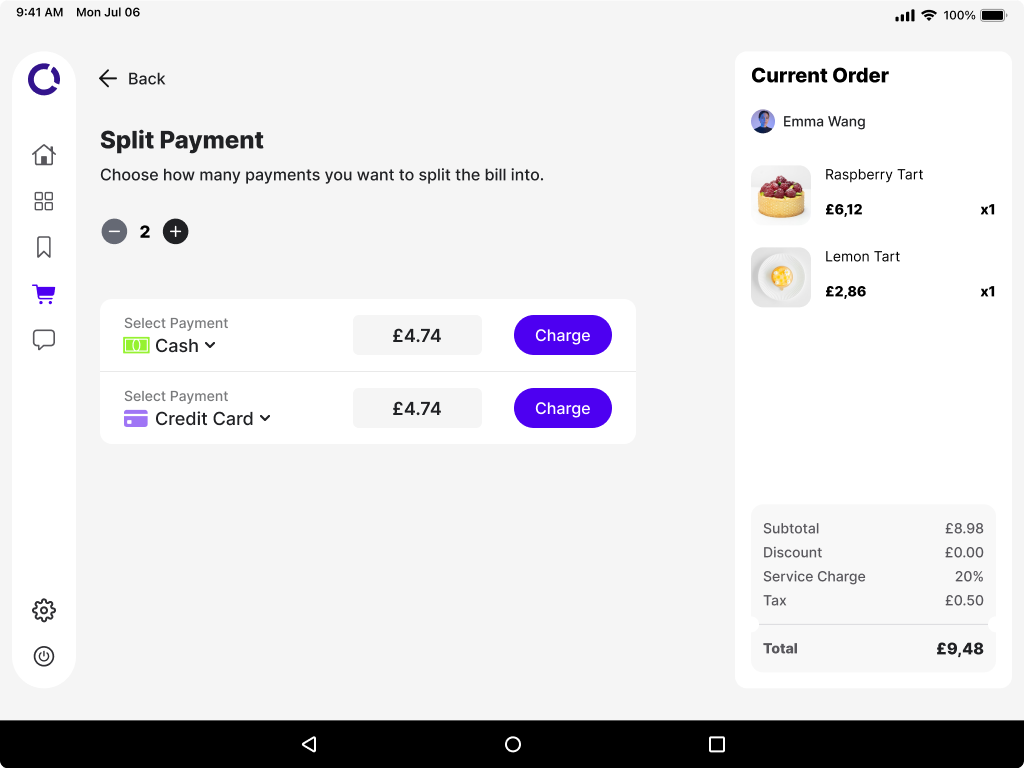
\includegraphics[width=0.9\linewidth]{HCI/images/split_payment.png}
    \caption{https://brightinventions.pl/blog/payment-point-of-sale-design-ui-ux/}
    \label{fig:Split_payment}
\end{figure}
\noindent
In the \cref{fig:Split_payment} interface design provides an interface to divide the bill into multiple payments and select different payment methods for each part, that can be adjusted. [\cref{N1-10}: N10]

\end{document}
